\section{Bipolartransistoren}
	\subsection{Schaltungen}
		\begin{figure}[h]
			\begin{subfigure}{0.3\textwidth}
			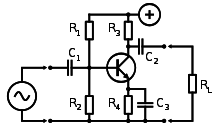
\includegraphics[width=\textwidth]{images/emitterschaltung}
			\begin{center}
			\caption{Emitterschaltung mit Arbeitspunkteinstellung}
			\end{center}
			\end{subfigure}
			\begin{subfigure}{0.3\textwidth}
			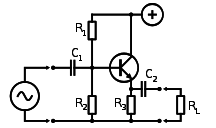
\includegraphics[width=\textwidth]{images/kollektorschaltung}
			\begin{center}
			\caption{Kollektorschaltung}
			\end{center}
			\end{subfigure}
			\begin{subfigure}{0.3\textwidth}
			\begin{center}
			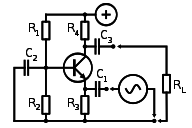
\includegraphics[width=\textwidth]{images/basisschaltung}
			\caption{Basisschaltung}
			\end{center}
			\end{subfigure}
		\end{figure}
		
		\begin{figure}[h]
			\begin{subfigure}{0.5\textwidth}
			%\input{images/kleinsignal}
			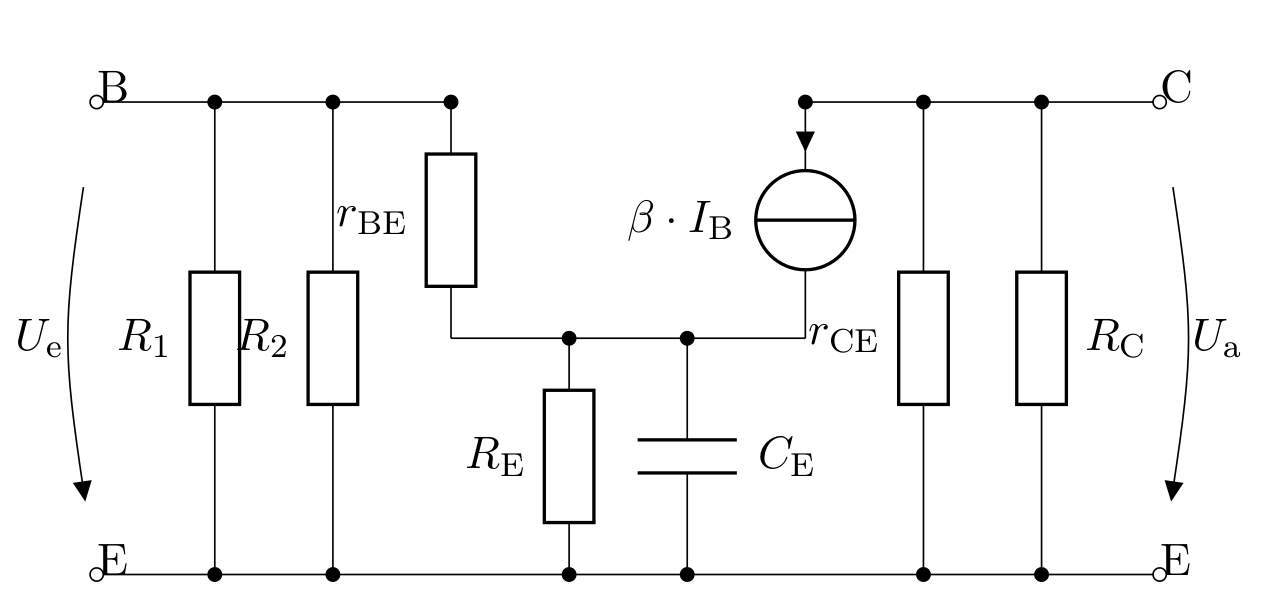
\includegraphics[width=\textwidth]{images/kleinsignal}
			\caption{Kleinsignalersatzschaltbild}
			\end{subfigure}
			\begin{subfigure}{0.5\textwidth}
			%\input{images/gl}
			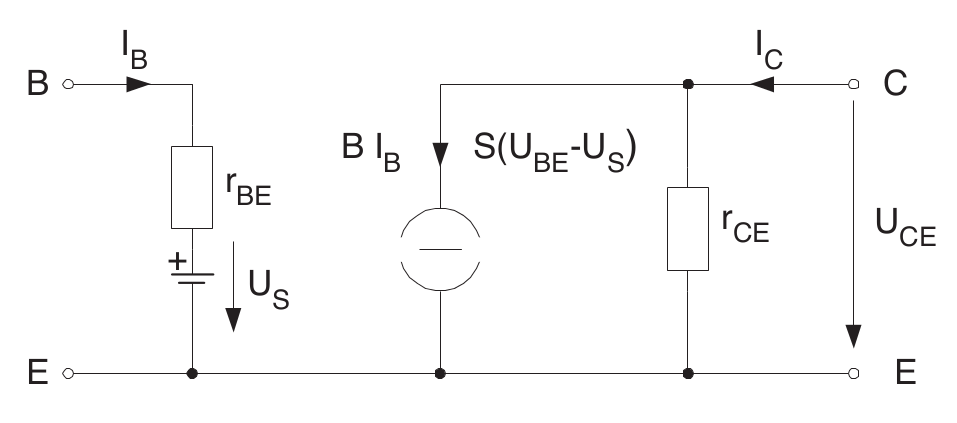
\includegraphics[width=\textwidth]{images/gleichstrom}
			\caption{Gleichstromersatzschaltbild}
			\end{subfigure}
		\end{figure}

	\subsection{Formeln}
		\subsubsection{Ströme}
			\begin{align*}
				I_{\mathrm{C}}&=B\cdot I_{\mathrm{B}} 
				& I_{\mathrm{B}}&=I_{\mathrm{S}}\cdot\left(e^{\frac{U_{\mathrm{BE}}}{U_{\mathrm{T}}}}-1\right) 
				& I_{\mathrm{E}}=I_{\mathrm{C}}+I_{\mathrm{B}} 
			\end{align*}
			\begin{table}[h]
			\begin{tabular}{ll}
			$I_{\mathrm{C}}\dots$ Kollektorstrom & $U_{\mathrm{T}}\dots$ Temperaturspannung, $86\mu\mathrm{V}\cdot\nicefrac{T}{\mathrm{K}}$, 26mV bei Raumtemperatur (300K)\\
			$I_{\mathrm{B}}\dots$ Basisstrom & $U_{\mathrm{BE}}\dots$ Basis-Emitterspannung, siehe Schaltbild
\\
			$I_{\mathrm{E}}\dots$ Emitterstrom & \\
			\end{tabular}
			\end{table}

		\subsubsection{Widerstände}
			\begin{align*}
				r_{\mathrm{BE}}\approx\frac{\Delta U_{\mathrm{BE}}}{\Delta I_{\mathrm{B}}}=\frac{U_{\mathrm{T}}}{I_{\mathrm{B}}} 
				&& r_{\mathrm{CE}}&=\frac{\Delta U_{\mathrm{CE}}}{\Delta I_{\mathrm{C}}}
			\end{align*}
			\begin{table}[h]
			\begin{tabular}{ll}
			$r_{\mathrm{BE}}\dots$ Basis-Emitter-Widerstand & $r_{\mathrm{CE}}\dots$ Kollektor-Emitter-Widerstand\\
			\end{tabular}
			\end{table}

		\subsubsection{Verstärkungen}
			\begin{align*}
				S&=\frac{\mathrm{d}I_{\mathrm{C}}}{\mathrm{d}U_{\mathrm{BE}}}\approx\frac{\Delta I_{\mathrm{C}}}{\Delta U_{\mathrm{BE}}}=\frac{I_{\mathrm{C}}}{U_{\mathrm{T}}} 
				& \beta\approx\frac{\Delta I_{\mathrm{C}}}{\Delta I_{\mathrm{B}}}
			\end{align*}
		
		\subsubsection{Early-Effekt}
			\begin{align*}
				I_{\mathrm{C}}&=B\cdot I_{\mathrm{B}}\cdot(1+\lambda U_{\mathrm{CE}})=B\cdot I_{\mathrm{B}}+\frac{U_{\mathrm{CE}}}{r_{\mathrm{CE}}} 
				& r_{\mathrm{CE}}&=\frac{\Delta U_{\mathrm{CE}}}{\Delta I_{\mathrm{C}}}=\frac{U_{\mathrm{y}}+U_{\mathrm{CE}}}{I_{\mathrm{C}}}=\frac{U_{\mathrm{y}}}{B\cdot I_{\mathrm{B}}}
				& \frac{1}{\lambda} &= U_{\mathrm{y}}
			\end{align*}

			$U_{\mathrm{y}}\dots$ Early-Spannung, ihr Fehlen weist auf Vernachlässigung des Early-Effekts hin $\Leftrightarrow$ kein $r_{\mathrm{CE}} \Leftrightarrow$ Transistor idealer Leiter

		\subsubsection{Emitterschaltung}
			\begin{align*}
				U_{\mathrm{B}}&=U_{\mathrm{CE}}+I_{\mathrm{C}}\cdot R_{\mathrm{C}} 
				& U_{\mathrm{a}}&=U_{\mathrm{CE}} & \Delta U_{\mathrm{a}}&=-\Delta I_{\mathrm{C}}\cdot R_{\mathrm{C}} 
				& S=\frac{\Delta I_{\mathrm{C}}}{\Delta U_{\mathrm{BE}}}\\
				\Delta U_{\mathrm{a}}&=-\Delta U_{\mathrm{e}}\cdot S\cdot R_{\mathrm{C}} 
				& v_{\mathrm{u}}&=\frac{\Delta U_{\mathrm{a}}}{\Delta U_{\mathrm{e}}}=-S\cdot R_{\mathrm{C}}
			\end{align*}
			\begin{table}[h]
			\begin{tabular}{ll}
			$S\dots$ Steilheit & $v_{\mathrm{u}}\dots$ Spannungsverstärkung\\
			$U_{\mathrm{a}}\dots$ Ausgangsspannung & $U_{\mathrm{e}}\dots$ Eingangsspannung\\
			\end{tabular}
			\end{table}
